\documentclass[journal,10pt]{IEEEtran}
\usepackage{graphicx}
\usepackage{booktabs}
\usepackage{amsmath,amssymb}
\usepackage{array}
\usepackage{cite}
\usepackage{url}
\usepackage{xcolor}
\graphicspath{{figures/}}
\hyphenation{dis-agree-ment inter-po-la-tion re-con-struc-tion}

\begin{document}
\title{Measurement Overlap Governs Disagreement-Based Reliability in Deterministic MRI Slice Interpolation}
\author{Anonymous Authors% Author names, affiliations, funding, and corresponding author required before submission.
}
\markboth{IEEE Transactions on Medical Imaging, Manuscript Under Preparation}{}
\maketitle

\begin{abstract}
Deterministic through-plane MRI interpolation can produce plausible missing slices without indicating when they are inaccurate. Disagreement between reconstructions is a natural retrospective reliability signal, but it observes only differences between their errors and can miss common-mode failures. We test the hypothesis that measurement overlap controls this blindness. Two frozen neural interpolators (HAT and SwinIR) reconstructed identical missing physical planes from either disjoint $\times4$ anchor lattices or the same anchors under a maximal-overlap order-reversal control. Dense targets were used only to synthesize retrospective alternative acquisitions and evaluate error. On 24 fastMRI brain T2 cases, zero-overlap disagreement correlated more strongly with target error than maximal-overlap disagreement (Spearman difference 0.355; case-clustered 95\% CI, 0.225--0.557). On 22 NingXia knee T2 series from eight patients, the difference was 0.193 (patient-clustered 95\% CI, 0.113--0.336). Effects remained positive for each architecture, while linear and cubic interpolators independently produced case-level correlations of 0.958--0.977 under disjoint sampling. Across frozen analyses, shared consensus error accounted for median 80.9\% and 86.5\% of squared error. Auxiliary IXI brain T2 results (115 cases) showed highly architecture-consistent difficulty but did not enter the controlled overlap test. These findings support a scoped design principle: reliability contexts should reduce shared error-generating measurements rather than merely maximize output diversity. Low disagreement cannot certify correctness.
\end{abstract}

\begin{IEEEkeywords}
Magnetic resonance imaging, slice interpolation, image reconstruction, reliability, uncertainty estimation, consistency, sampling.
\end{IEEEkeywords}

\section{Introduction}
\IEEEPARstart{A}{nisotropic} magnetic resonance imaging (MRI) volumes often have substantially coarser through-plane than in-plane resolution. Interpolating unacquired slices can ease visualization and downstream volumetric processing, and modern slice-synthesis networks improve over classical interpolation in many settings \cite{peng2020saint,song2024i3net}. Yet a deterministic interpolator normally returns one image, even when the acquired anchors do not constrain the missing anatomy sufficiently. A deployment-facing reliability signal must therefore identify likely failure without accessing the dense target that is missing in practice.

Model ensembles, stochastic sampling, test-time augmentation (TTA), and cross-context consistency estimate reliability from variation among plausible outputs \cite{gal2016dropout,lakshminarayanan2017ensembles,edupuganti2021uncertainty,narnhofer2022bayesian}. Their common premise is useful but one-sided: disagreement witnesses that at least one prediction differs, whereas agreement need not imply correctness. If two reconstructions inherit the same smoothing, boundary limitation, or anchor-induced bias, subtracting them removes the very error one wishes to detect. This issue is especially relevant to interpolation because nearby reconstruction contexts can reuse the same acquired slices.

We investigate measurement overlap as a control variable for error observability (Fig.~\ref{fig:concept}). The same missing physical plane is reconstructed twice at the same nominal factor. In one condition, the two contexts draw from phase-shifted $\times4$ anchor lattices with no shared slices. In the maximal-overlap control, they use the identical anchor lattice but reverse its through-plane order before mapping the output back. Case, target, model, plane, evaluation support, and number of measurements remain paired. The control has a known limitation---reversal changes ordering---so we interpret it as a mechanistic retrospective intervention, not a complete causal identification of overlap alone.

The study makes four contributions. First, it formalizes consensus blindness as cancellation of aligned reconstruction errors and links the observable fraction of squared error to context diversity. Second, it conducts a target-preserving measurement-overlap intervention in brain and knee T2 MRI, with corrected patient-level inference for the multi-series knee cohort. Third, it tests architecture, analytical-interpolator, raw-diversity, and stable-wrong boundaries. Fourth, it evaluates a methodological consequence: whether disjoint-context disagreement retrospectively ranks the benefit of denser sampling. All claims concern deterministic MRI slice interpolation; we do not claim calibrated uncertainty, prospective acquisition benefit, or clinical safety. The resulting contribution is therefore a reliability-design study rather than a new reconstruction backbone: it asks which measurements must change before consistency can carry useful evidence about error.

\begin{figure}[t]
\centering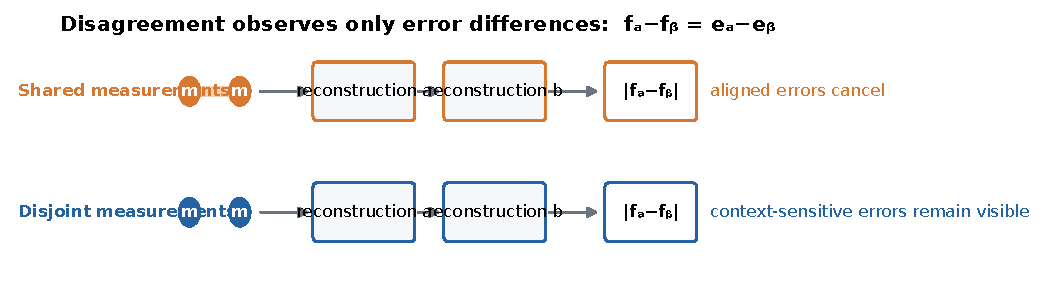
\includegraphics[width=\columnwidth]{fig1_concept.pdf}
\caption{Consensus blindness. When contexts reuse error-generating measurements, aligned errors cancel in output disagreement. Disjoint contexts can reveal a larger context-sensitive component, but agreement still cannot certify correctness.}
\label{fig:concept}
\end{figure}

\section{Related Work}
\subsection{MRI Slice Synthesis and Interpolation}
Classical linear and cubic splines estimate missing samples from smoothness assumptions \cite{deboor1978splines}. Deep slice-synthesis methods instead learn anatomical priors. SAINT conditions synthesis on spatial position and supports variable upsampling factors \cite{peng2020saint}; I3Net combines inter- and intra-slice information for medical slice synthesis \cite{song2024i3net}. These approaches primarily optimize reconstruction fidelity. Our question is complementary: given a frozen deterministic interpolator, which target-preserving contexts expose its retrospective error?

\subsection{Reconstruction Uncertainty and Reliability}
MRI reconstruction uncertainty has been estimated through variational latent models, SURE, Bayesian parameter distributions, and posterior sampling \cite{edupuganti2021uncertainty,narnhofer2022bayesian}. In neuroimage enhancement, predictive uncertainty has also been evaluated against errors and distribution shift \cite{tanno2021uncertainty}. These methods address probabilistic reconstruction or learned uncertainty. We do not estimate a calibrated posterior; we study why a broad class of output-disagreement signals can be blind when errors are shared.

\subsection{Consistency, Diversity, and Shared Error}
Deep ensembles and stochastic perturbations use diversity as evidence of uncertainty \cite{lakshminarayanan2017ensembles,gal2016dropout}. Ensemble theory emphasizes that diversity interacts with, rather than replaces, individual predictor accuracy \cite{brown2005diversity,ortega2022diversity}. Self-consistency also has a long history in MRI reconstruction, including measurement consistency in SPIRiT \cite{lustig2010spirit}. Our closest distinction is intervention-level: we manipulate overlap of acquired through-plane measurements for the same target and quantify reliability ranking, rather than interpreting arbitrary output dispersion as uncertainty.

\section{Theory: Consensus Error and Disagreement Blindness}
Let $y$ be a missing target slice and let two deterministic contexts produce
\begin{equation}
 f_a=y+e_a,\qquad f_b=y+e_b.
\end{equation}
Their difference contains no target term:
\begin{equation}
 f_a-f_b=e_a-e_b,
\end{equation}
and squared disagreement satisfies
\begin{equation}
 \|e_a-e_b\|^2=\|e_a\|^2+\|e_b\|^2-2\langle e_a,e_b\rangle. \label{eq:cov}
\end{equation}
Positive error alignment therefore reduces observable disagreement at fixed marginal error energy. Define the context mean $\bar e=(e_a+e_b)/2$ and half-difference $\delta=(e_a-e_b)/2$. The exact identity
\begin{equation}
 \tfrac12(\|e_a\|^2+\|e_b\|^2)=\|\bar e\|^2+\|\delta\|^2 \label{eq:decomp}
\end{equation}
separates shared consensus error from context-observable diversity. This is an algebraic decomposition, not a calibrated uncertainty partition. It also does not identify which reconstruction is wrong.

An immediate boundary follows from the common-mode case $e_a=e_b=c$. Then $\delta=0$ and disagreement vanishes for every nonzero $c$, while the complete error remains in $\bar e=c$. Conversely, if $e_a=-e_b$, the mean error cancels and all paired energy is observable. Real interpolation contexts lie between these extremes. A reliability intervention is useful only insofar as it rotates or decorrelates relevant error components; changing output appearance without changing their direction relative to the target need not improve observability.

For any metric $d$ obeying the triangle inequality,
\begin{equation}
 d(f_a,f_b)\leq d(f_a,y)+d(f_b,y).
\end{equation}
Thus large disagreement lower-bounds the sum of errors only in a one-sided sense, while small disagreement gives no upper bound. A pair can be stably wrong with $e_a\approx e_b\neq0$. Equation~\eqref{eq:cov} motivates the hypothesis that reducing overlap of error-generating measurements decreases $\langle e_a,e_b\rangle$ and makes error more observable.

\section{Measurement-Overlap Hypothesis}
A \emph{target-preserving context} is a set of acquired anchors and reconstruction operations that predicts the same physical missing plane. Measurement overlap is the number of identical acquired slices shared by the two bracketing contexts. At factor four, phase-0 anchors are $z=0,4,8,\ldots$ and phase-2 anchors are $z=2,6,10,\ldots$. Targets with $z\bmod4\in\{1,3\}$ are missing from both grids, and the two grids share no anchors (Fig.~\ref{fig:design}).

The maximal-overlap control uses the phase-0 anchors in both contexts, reverses the sparse sequence for one run, and maps its prediction back to physical $z$. It shares two bracketing anchors for each interior target. Our prespecified directional prediction is that greater overlap increases error alignment, lowers the observable error fraction, and weakens ranking of target error by disagreement. Only the final ranking comparison was available in the frozen TMI evidence; covariance-arrow tests and cleaner flip controls are reserved for the separated exploratory conference branch.

\begin{figure}[t]
\centering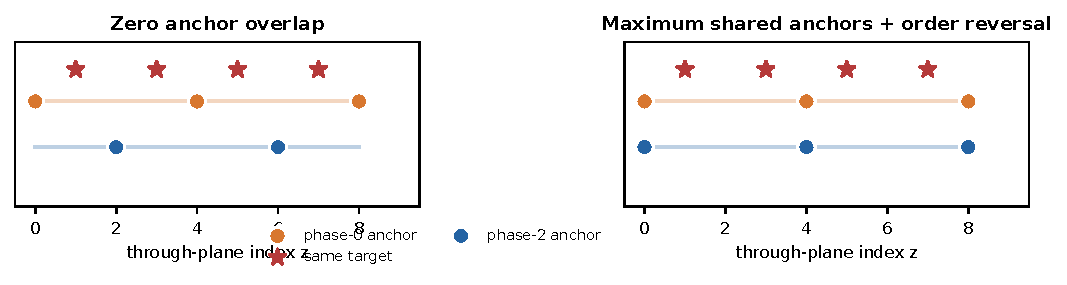
\includegraphics[width=\columnwidth]{fig2_design.pdf}
\caption{Paired $\times4$ design. Stars mark the same evaluated missing targets. The zero-overlap condition changes the phase lattice; the maximal-overlap control reuses the phase-0 anchors under order reversal.}
\label{fig:design}
\end{figure}

\section{Materials and Methods}
\subsection{Data and Units of Analysis}
Table~\ref{tab:data} summarizes the frozen cohorts. The expanded fastMRI-brain-T2 subset contained 160 NIfTI volumes split 112/24/24; all controlled analyses used the 24-case test partition. The underlying fastMRI resource is public and deidentified \cite{zbontar2018fastmri,knoll2020fastmri}. NingXia-T2 contained 22 knee MRI series from eight patients. Predictions were strictly out of fold under eight patient-group folds; all new inferential resampling uses the patient prefix rather than treating 22 series as independent. This corrects the historical record without changing stored point estimates. IXI-T2 \cite{ixi_dataset} contributed 115 held-out brain MRI cases at $\times4$ to frozen auxiliary analyses of architecture-independent difficulty and input-derived difficulty. It did not enter the zero-versus-maximal overlap comparison reported here.

Inclusion required matching case identity, finite arrays, equal in-plane dimensions, and a valid NIfTI affine. Generated planes were matched in world coordinates by their affine-derived origins within 0.001~mm. Acquired anchors were excluded. No registration or post-validation resampling was allowed.

\begin{table}[t]
\caption{Cohorts and frozen experimental roles}
\label{tab:data}\centering
\begin{tabular}{p{1.05cm}p{.72cm}p{1.25cm}p{.58cm}p{2.3cm}}
\toprule
Cohort & Site & Unit $N$ & $r$ & Role \\
\midrule
fastMRI T2 & brain & 24 cases & 2/4/6 & Main overlap; models; analytical; benefit \\
NingXia T2 & knee & 8 patients / 22 series & 2/4/6 & OOF main overlap and replication \\
IXI T2 & brain & 115 cases & 4 & Auxiliary frozen difficulty replication \\
\bottomrule
\end{tabular}
\end{table}

\subsection{Reconstruction Methods}
The decisive controlled experiment used frozen 2.5-D HAT and SwinIR interpolators. They process adjacent acquired slices and synthesize the missing interval; checkpoints and predictions were fixed before the Plan-4 overlap analyses. I3Net was included in the broader frozen factor and TTA comparisons but excluded from the disjoint phase intervention because most fastMRI volumes provided only three phase-shifted anchors while the frozen implementation required four; we did not pad uncovered outputs. Linear and cubic interpolation were evaluated as non-neural families under the same disjoint phase construction.

\subsection{Reliability Scores and Endpoints}
For paired predictions $a,b$, the primary plane score was mean absolute disagreement on the deployment mask $|a|>0.01\max|a|$. The retrospective endpoint was mean absolute error of the stored phase-0 prediction on that identical mask. Dense targets entered only phase-grid simulation and evaluation, never the reliability score. Examination or model--series scores were medians across matched generated planes.

Frozen secondary comparators included: (i) target-excluded committee disagreement; (ii) Physical Consistency (PC-v1), the median absolute difference among NIfTI-affine matched predictions at $\times2$, $\times4$, and $\times6$; (iii) four-view flip-TTA; and (iv) adjacent-anchor RMSE, computed before reconstruction. Ranking used Spearman correlation and normalized area under the risk--coverage curve (nAURC). The latter normalizes empirical selective risk between oracle and reverse-oracle rankings. Densification benefit was the realized reduction in reconstruction MAE from stored $\times4$ to $\times2$ outputs.

Spearman correlation measures ordering rather than absolute calibration and is invariant to monotone score transforms. Risk--coverage analysis complements it by asking whether removing the highest-scored observations actually reduces retained error. These endpoints were chosen because disagreement scales differ substantially by cohort and model; no pooled intensity threshold or cross-cohort uncertainty calibration is assumed.

\subsection{Statistical Analysis}
Repeated planes, factors, and architectures were not treated as independent patients. Primary intervals used 5,000 cluster bootstrap replicates, resampling 24 fastMRI cases or eight NingXia patient groups with all subordinate observations retained. The PC--TTA comparison used whole-cluster score swaps; its historical NingXia 22-series permutation was superseded by a 10,000-swap patient-group analysis. Plane-level correlations describe ranking across evaluated planes, with clustered intervals quantifying sensitivity to independent-unit sampling. Analyses were paired by dataset, case, model, and plane. No multiple-comparison-adjusted universal superiority claim is made.

The distinction between analysis and sampling units is essential for NingXia: a series can contribute multiple planes and a patient can contribute multiple series, but neither creates an additional independent patient. Accordingly, resampling a patient carries all of its series, models, and planes together. The manuscript reports pooled plane ranking only when the corresponding interval respects that hierarchy.

\section{Experiments and Results}
\subsection{Consensus Error Dominates Context Diversity}
Applying Eq.~\eqref{eq:decomp} to frozen paired context errors assigned median 80.9\% of total squared error to the shared consensus component on fastMRI and 86.5\% on NingXia; observable diversity accounted for 19.1\% and 13.5\% (Fig.~\ref{fig:decomp}a). The identity residual was negligible relative to squared-error scale. Consistent difficulty also extended beyond a single pair: median pairwise error-rank correlation was 0.961 among 11 fastMRI neural models and 0.991 among six methods on the 115-case IXI panel. These descriptive results establish a substantial common component but do not prove that every shared error originates from measurements.

\subsection{Controlled Measurement-Overlap Intervention}
Figure~\ref{fig:main} and Table~\ref{tab:main} report the primary comparison. On fastMRI, zero-overlap disagreement had plane-level Spearman $\rho=0.960$ with phase-0 MAE, versus 0.605 for the maximal-overlap reversal control, a difference of 0.355 (case-clustered 95\% CI, 0.225--0.557). On NingXia, the corresponding values were 0.891 and 0.699, a difference of 0.193. Correct resampling of eight patient groups gave a 95\% CI of 0.113--0.336. Endpoint differences were exactly zero because both scores were evaluated against the same stored phase-0 error.

\begin{figure}[t]
\centering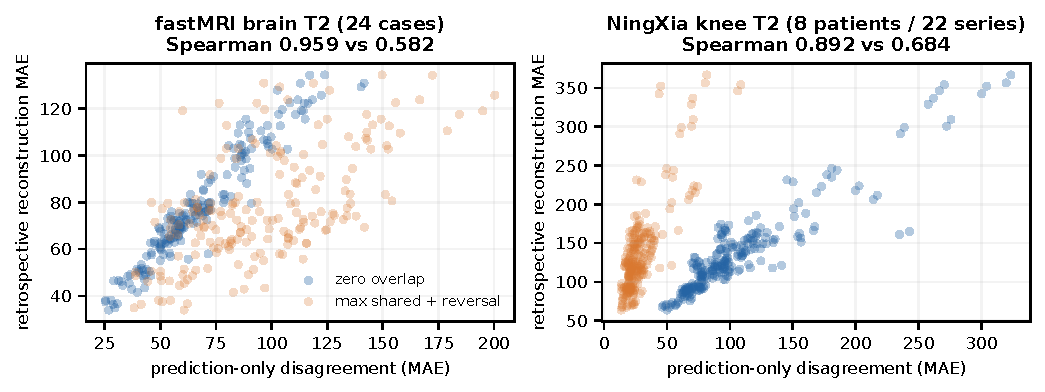
\includegraphics[width=\columnwidth]{fig3_main_overlap.pdf}
\caption{Same-target controlled result. Each point is a model--plane observation; inference is clustered by case (fastMRI) or patient (NingXia). Zero-overlap scores rank retrospective MAE better than the shared-anchor reversal control.}
\label{fig:main}
\end{figure}

\begin{table}[t]
\caption{Zero versus maximal shared-anchor reliability}
\label{tab:main}\centering
\begin{tabular}{p{1.1cm}p{1.0cm}rrrr}
\toprule
Cohort & Model & $\rho_0$ & $\rho_{\max}$ & $\Delta\rho$ & 95\% CI \\
\midrule
fastMRI & pooled & .960 & .605 & .355 & [.225,.557] \\
 & HAT & .967 & .626 & .340 & [.205,.559] \\
 & SwinIR & .958 & .582 & .375 & [.233,.586] \\
NingXia & pooled & .891 & .699 & .193 & [.113,.336] \\
 & HAT & .892 & .764 & .128 & [.025,.233] \\
 & SwinIR & .890 & .632 & .258 & [.133,.513] \\
\bottomrule
\end{tabular}
\end{table}

\subsection{Architecture and Analytical Generalization}
The effect was positive for HAT and SwinIR separately in both cohorts (Table~\ref{tab:main}; Fig.~\ref{fig:generalization}a). Under zero-overlap grids, classical linear and cubic interpolation also produced strong case-level reliability: Spearman correlations were 0.977 and 0.974 on fastMRI and 0.958 and 0.967 on NingXia (Fig.~\ref{fig:generalization}b). These analytical results show that the useful witness is not uniquely tied to neural stochasticity. Because the analytical experiment lacked a frozen matched maximal-overlap comparator, it supports disjoint-context generality rather than the overlap contrast itself.

\begin{figure}[t]
\centering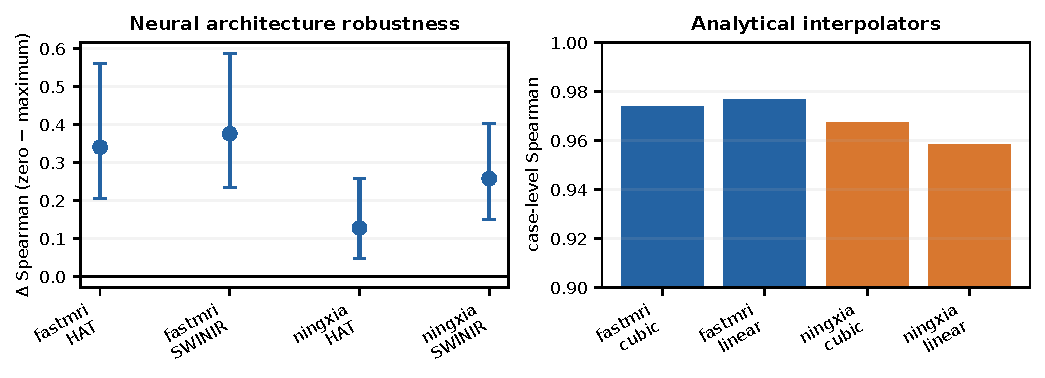
\includegraphics[width=\columnwidth]{fig4_generalization.pdf}
\caption{Generalization. (a) Architecture-specific zero-minus-maximal rank-correlation differences. (b) Case-level disjoint-context correlation for linear and cubic interpolation. Historical NingXia neural intervals were recomputed by eight patient clusters.}
\label{fig:generalization}
\end{figure}

\subsection{Raw Diversity Is Not Sufficient}
On fastMRI, zero-overlap median raw disagreement was only 59.1\% (HAT) and 77.2\% (SwinIR) of maximal-overlap disagreement, yet its error ranking was substantially stronger. Thus a condition can produce larger output differences while being a worse reliability ranker. NingXia showed the opposite magnitude ordering, so raw scale is cohort dependent. The conclusion is deliberately narrow: larger raw output diversity is neither necessary nor sufficient for better ranking in these controls.

\subsection{Retrospective Predictive Consequence}
Disjoint $\times4$ disagreement predicted the realized $\times4\rightarrow\times2$ reduction in reconstruction MAE with $\rho=0.811$ (95\% CI, 0.592--0.904) on 48 fastMRI model--case units and $\rho=0.626$ on 44 NingXia model--series units; patient-cluster correction gave 95\% CI 0.200--0.844. At a prespecified top-25\% retrospective densification budget, score-ranked MAE reductions were 33.36 versus 21.37 for random selection on fastMRI and 35.39 versus 24.25 on NingXia (Fig.~\ref{fig:decomp}b). The fastMRI policy captured 97.6\% of the oracle gain above random; NingXia captured 76.5\%. This is retrospective predictive validity using already dense targets, not prospective or clinical acquisition optimization.

\begin{figure}[t]
\centering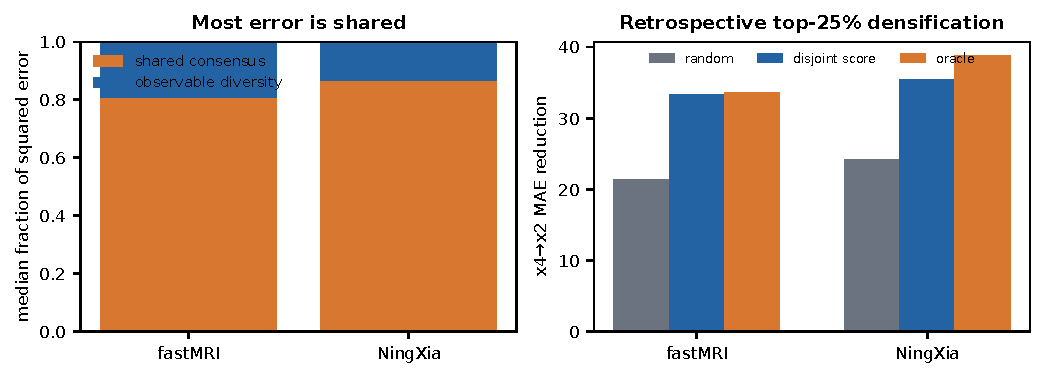
\includegraphics[width=\columnwidth]{fig5_decomposition_consequence.pdf}
\caption{Error decomposition and consequence. (a) Most paired squared error is shared. (b) At a fixed retrospective 25\% budget, disjoint-score selection yields larger stored $\times4\rightarrow\times2$ MAE reduction than random selection and approaches the oracle.}
\label{fig:decomp}
\end{figure}

\subsection{Failure Boundary and Negative Results}
Agreement is not a correctness certificate. Frozen localization analyses found 14 NingXia planes simultaneously in the lowest PC quartile and highest error quartile; 12 occurred at the first generated $\times4$--$\times6$ position, suggesting shared boundary-context failure. Controlled common blur similarly reduced variation while preserving error. Conversely, no natural stable-wrong plane met the same quartile rule in fastMRI, so prevalence did not replicate.

Input-side difficulty also had a mixed interpretation. Adjacent-anchor RMSE predicted raw error across fastMRI ($\rho=0.719$), NingXia ($\rho=0.780$), and IXI ($\rho=0.982$ across six methods), but correlations with range-normalized error fell to 0.503, 0.465, and 0.251. A fully normalized feature was robust only on IXI ($\rho=0.644$). A curvature--spacing model improved held-out fastMRI prediction over spacing alone, but absolute transfer to NingXia failed. These negative results reject a universal input-only error law.

Finally, PC beat flip-TTA in all nine frozen fastMRI profiles (mean $\Delta$nAURC $=-0.034$, case-clustered permutation $p=0.0035$). Although all nine NingXia point estimates favored PC, correcting the independent unit to eight patients changed the mean difference to $-0.047$ with $p=0.742$. We therefore do not claim statistically supported PC superiority on NingXia, nor superiority over arbitrary perturbation families.

\section{Discussion}
The experiments support a mechanistic account of disagreement blindness in deterministic MRI interpolation. Reconstruction contexts can share a large consensus error, and Eq.~\eqref{eq:cov} shows why aligned errors disappear under subtraction. The controlled phase-grid intervention changes the acquired information supporting the same target. Disjoint grids rank error better than a same-anchor reversal context across two anatomies and two neural architectures, while analytical interpolation provides an estimator-family replication. The result is stronger than observing that perturbations produce different outputs: the paired endpoint is fixed, measurement identity is recorded, and a raw-magnitude control demonstrates that more output variation is not itself the operative goal.

The findings also clarify what disagreement can and cannot mean. High disjoint-context disagreement is useful evidence of context-sensitive failure. Low disagreement is ambiguous because both contexts may share bias. In practice, reliability systems should therefore seek contexts that reduce dependence in error-generating information, while retaining explicit stable-wrong safeguards. This principle complements probabilistic reconstruction: even posterior or ensemble samples can underestimate risk if their construction does not vary the source of shared error.

This perspective separates three properties that are often conflated. \emph{Diversity} is the observed distance between outputs. \emph{Observability} is the fraction of actual paired error that survives in that distance. \emph{Calibration} maps a score to a probabilistic or absolute error statement. Our experiments address the first two and show that diversity alone does not determine observability; they do not establish the third. Consequently, a disjoint-context score can rank difficult examinations while remaining unsuitable for statements such as ``this slice has less than a specified error.''

The retrospective densification result offers a methodological consequence. Cases with larger disjoint disagreement tended to realize larger gains from denser stored sampling. That relationship is promising for acquisition-allocation research because the score itself uses only alternative sparse contexts. However, constructing two disjoint $\times4$ grids consumes the union of measurements equivalent to denser coverage in this simulation. A practical policy would require a lower-cost pilot, sequential sampling, or a pre-inference surrogate evaluated prospectively. The present study does not solve that deployment problem.

The controlled intervention also has an imaging-specific interpretation. Through-plane anchors are not exchangeable generic augmentations: their physical locations determine both interpolation distance and the anatomical information available to a reconstruction. Preserving the physical target and evaluation support while recording anchor identity is therefore necessary for assigning a measurement-overlap interpretation. This requirement explains why ordinary flip-TTA, architecture committees, and phase-grid comparisons answer related but nonidentical reliability questions.

The IXI evidence adds scale and a second brain cohort to the broader observation that interpolation difficulty is largely shared across methods. It does not constitute an IXI replication of the frozen overlap intervention, and we intentionally keep newer IXI overlap experiments outside this manuscript's evidence freeze. This separation prevents exploratory upgrades from silently strengthening a journal claim.

\section{Limitations}
All phase grids are retrospective simulations from dense volumes; no scanner prospectively changed its sampling. The primary controlled evidence includes one brain T2 cohort and one small knee T2 cohort; NingXia has only eight independent patient groups despite 22 series. IXI contributes auxiliary difficulty evidence, not the main intervention. Only HAT and SwinIR support the decisive neural phase-grid experiment; I3Net was infeasible without artificial padding. The maximal-overlap reversal control changes through-plane ordering and may invoke equivariance effects beyond overlap. A strict multi-level overlap ladder with fixed two-anchor distances is geometrically infeasible; cleaner controls remain exploratory.

Intensity-derived MAE and disagreement require comparable preprocessing within each paired profile and do not support cross-cohort absolute calibration. The study has no reader task, pathology label, clinical endpoint, prospective adaptive acquisition, or safety analysis. It cannot identify which output is wrong, guarantee accuracy from agreement, or establish universal superiority over uncertainty estimators. Common-mode blur and boundary failures remain explicit counterexamples. Finally, parts of the evidence were generated after inspecting earlier results; except where a protocol was historically frozen, analyses are labeled exploratory rather than confirmatory.

\section{Ethics and Data Availability}
fastMRI and IXI are publicly accessible human-derived MRI resources; use here was retrospective and involved locally prepared deidentified images. The exact consent, institutional-review, and data-use wording for the particular fastMRI-brain and IXI releases must be copied from their governing records before submission. NingXia is an internal human MRI cohort. \textbf{[ETHICS INFORMATION REQUIRED FROM AUTHORS: approving or exempting institution, decision/approval identifier where applicable, consent or waiver, and permitted data-use statement.]}

Code, immutable historical experiment records, case-level manifests, and derived numerical outputs are organized in the accompanying repository. Raw public data remain under their source licenses; internal NingXia images are not redistributed. An anonymized repository URL and any sharing restrictions must be supplied before submission. No generative-AI content disclosure is asserted here; authors must add the disclosure required by current IEEE policy if applicable to manuscript preparation.

\section{Conclusion}
In deterministic MRI slice interpolation, disagreement observes differences between reconstruction errors, not error itself. Shared measurements can align errors and conceal them. Across paired brain and knee T2 experiments, target-preserving disjoint anchor grids ranked retrospective error more effectively than a maximal-shared-anchor reversal control, and the effect persisted across two neural architectures and analytical interpolation. The supported principle is narrow: design reliability contexts to reduce shared error-generating information. Agreement alone cannot certify correctness.

\bibliographystyle{IEEEtran}
\bibliography{references}
\end{document}
